\chapter{Sviluppo Back-end per l'inserimento di mappe}
\label{cap:chapter6}

\section{Programma AutoLoader}
 
Dal momento che tutti i formati di mappe erano stati testati ed integrati, riuscendo quindi ad avere per ognuna di loro un'implementazione funzionante lato front-end, ciò che rimaneva da fare, oltre che a migliorare l'integrazione tra front-end e back-end, era la realizzazione di un meccanismo che consentisse il caricamento automatico di tutte le mappe all'intero di GeoServer. Fino ad allora, infatti, soltanto alcune delle mappe erano state caricate, e quelle poche servivano ad avere un'implementazione funzionante per quei formati. Infatti, il front-end, anche se in maniera "hard coded", riusciva a richiedere le mappe nei protocolli WMTS (quando possibile), WMS e WFS al GeoServer, oltre che a supportare gli stili personalizzati nel formato SLD. 
\\In questa seconda fase di sviluppo, quindi, lo scopo del tirocinante è stato quello di realizzare un sistema, che prende il nome di AutoLoader, per il caricamento automatico di tutte le mappe all'interno di GeoServer.  Questo permetteva non solo di verificare che tutte le mappe funzionassero correttamente con le implementazioni da lui effettuate, ma anche di prepararle per l'integrazione all'interno del sistema stesso.

\subsection{Risoluzione del problema della Rest API}

L'idea principale dietro questo programma era quella di sviluppare un'applicazione in C\# che, sfruttando la REST API fornita da GeoServer, fosse in grado di creare automaticamente delle Workspace e degli Storage in cui caricare le mappe, per poi pubblicare tutti i layer presenti al loro interno. Per selezionare quali mappe caricare all'interno di GeoServer, si è deciso di far leggere al programma i dati da un file CSV, utilizzando come base di partenza quello realizzato dal candidato i primi giorni di tirocinio.
\\Il problema principale con questa implementazione è che le API fornite da GeoServer, come viene riportato dagli sviluppatori nella loro documentazione \cite{DocumentazioneGeoServerAPI}, presentano tutt'ora alcune criticità importanti che possono influenzare il suo utilizzo e la sua affidabilità. Innanzitutto, la specifica della REST API è rimasta alla versione di Swagger 2.0 e non è aggiornata al nuovo standard di OpenAPI 3.0. Ciò ha chiaramente comportato una peggiore comprensione e utilizzo dell'API stessa, ma sopratutto, viene fatto notare che i file di Swagger utilizzati per documentare l'API sono stati creati manualmente nel 2017 e non sono stati più aggiornati con l'evoluzione dell'infrastruttura del software: 
\begin{quote}
``Warning The API is documented as Swagger 2.0 files. However, these files have been written by hand back in 2017, and have not always been kept up to date with the evolution of the GeoServer configuration object structure. Also, they have not been tested for proper client generation, and will likely not work for that purpose. Take them only as a form of documentation.''
\end{quote}
\\L'utilizzo dell'API di GeoServer, purtroppo, è stata una parte cruciale durante questa fase di sviluppo, e questo problema ha rappresentato una sfida significativa, in quanto è stato necessario sistemare manualmente le richieste, al fine di poterle poi utilizzare correttamente.
\\~\\
Il tirocinante si è dunque dedicato allo studio del linguaggio di programmazione C\#, e alle API messe a disposizione dal server di mappe. Il lavoro è poi proseguito sviluppando un programma, inizialmente esterno al progetto, capace di contattare il servizio di GeoServer; quest'ultimo avviato localmente attraverso un container Docker.
\\Per comunicare con la sua REST API, anziché scrivere un programma da zero per gestire manualmente ogni richiesta HTTP, dovendo quindi realizzare per ciascuna di esse una struttura dati apposita (con cui gestire e manipolare le richieste), è stato deciso di utilizzare una libreria opportuna. Tale libreria, nota con il nome di NSwag, permette di contattare il servizio REST API in automatico, senza doversi preoccupare di fare tutto quello descritto precedentemente. Nel dettaglio, questa libreria richiede come input il file YAML che descrive la specifica della REST API, attraverso la quale NSwag genera una o più classi contenenti a loro interno dei metodi già implementati, permettendo così di contattare il servizio.
\\La struttura dell'API di GeoServer, come molte altre, era organizzata ad endpoint, ognuno dei quali forniva delle funzionalità diverse. In questo modo era quindi possibile per il tirocinante contattare solamente quelli che possedevano le funzionalità a lui interessate. Inoltre, ogni endpoint possedeva il file Yaml della loro specifica REST API, fondamentale a Nswag per generare i metodi e le classi sopra citate.
\\Il candidato ha quindi scelto i seguenti endpoint, essenziali per la realizzazione del programma AutoLoader: 
\begin{itemize}
    \item \verb|/workspace|: questo endpoint contiene le richieste HTTP necessarie per creare, modificare, o eliminare le workspace all'interno di GeoServer;
    \item \verb|/wmsstores|: in maniera analoga a quello precedente, questo contiene tutte le richieste HTTP utili per creare, modificare, o eliminare uno storage WMS all'interno di una Workspace;
    \item \verb|/wmslayers|: questo endpoint, invece, contiene le operazioni relative ai layer all'interno di uno storage WMS. Oltre alle operazioni di base (come negli endpoint precedenti), permette di richiedere l'elenco di tutti i layer pubblicati e non, oltre a consentire la loro pubblicazione;
    \item \verb|/datastores|: consente di eseguire operazioni su tutti gli altri storage diversi dallo storage WMS o WMTS. Ad esempio, viene utilizzato per operare su uno storage WFS, o per lavorare su uno storage che contiene uno Shapefile;
    \item \verb|/featuretypes|: questo endpoint, infine, offre tutte le operazioni per lavorare con le feature presenti all'interno di un data store. In maniera analoga a \verb|/wmslayers|, permette di richiedere l'elenco di tutte le feature pubblicate e non, oltre a consentirne la pubblicazione;
\end{itemize}
\\Dopo aver generato con successo le classi tramite NSwag, il tirocinante ha quindi iniziato a verificare se i metodi al loro interno funzionassero correttamente, procedendo, per ognuno di essi, ad invocarli all'interno del programma. Poiché la specifica riportata non rispettava minimamente ciò che il GeoServer richiedeva, i metodi così generati risultavano non funzionanti, costringendo così il tirocinante a doverli riparare. Per fare ciò, è ricorso all'uso del comando cURL e del software Postman, affinché potesse controllare, con l'avanzare dello sviluppo dell'applicazione, che tutte le richieste corrispondessero a quanto descritto nella documentazione di SwaggerUI. Nel caso in cui ci fossero state delle discrepanze tra le richieste e quanto documentato, quindi, il tirocinante sarebbe dovuto intervenire modificando manualmente il file YAML fornito. 
%un esempio di yaml malformato?
\\Successivamente, il candidato ha deciso creare una nuova classe in cui, seguendo il Wrapper Design Pattern, ha incapsulato tutti i metodi autogenerati da NSwag, riuscendo così ad avere una organizzazione più pulita del codice e degli argomenti passati alle funzioni. All'interno di questa classe (che è diventata quella principale del programma), il tirocinante ha poi aggiunto dei nuovi metodi che consentivano di eseguire delle operazioni automatiche che normalmente non erano fornite dalla REST API stessa. Tra questi, il più importante è stato il metodo \verb|AddNewMapAsync()|, il quale consentiva di caricare automaticamente una mappa all'interno di GeoServer.

\subsection{Risoluzione del problema di identificazione dei Layer}

Normalmente, quando si vogliono caricare delle mappe al suo interno, si passa o un servizio di mappe esterno (come un server WMS), oppure si carica direttamente un file geospaziale (come ad esempio uno Shapefile): in entrambi casi, può succedere che al loro interno ci possano essere più layer da pubblicare. 
\\Il GeoServer, per diversificare quest'ultimi, utilizza come identificativo esattamente il nome del layer associato al nome della workspace in cui si trova (invece che utilizzare, banalmente, un numero come id oppure una funzione di hashing). Ad esempio, se viene caricata una mappa all'interno di GeoServer, quest'ultima verrà identificata nel seguente modo: \verb|nome_workspace:nome_layer|.
\\Durante il caricamento delle mappe è capitato che diverse fonti avessero al loro interno dei layer con lo stesso nome, portando quindi ad un errore nel loro inserimento, poiché non potevano esistere più layer con lo stesso nome associati alla medesima workspace.
\\Per evitare questo problema, il tirocinante ha proposto di creare una workspace separata per ogni servizio di mappe, invece di inserire tutti i servizi nella stessa workspace con i loro rispettivi layer. Di seguito è mostrata un'immagine che descrive meglio come è stata organizzata la gestione delle mappe all'interno di GeoServer.
\\~\\
\begin{minipage}{0.5\textwidth}
\dirtree{%
.1 Single Workspace.
.2 WMS Storage.
.3 layer 1.
.3 layer 2.
.3 layer **.
.2 WMS Storage 2.
.3 layer 1.
.3 layer 2.
.3 layer **.
.2 ShapeFile Storage.
.3 layer 1.
.3 layer 2.
.3 layer **.
}
\textbf{Old File Structure}
\end{minipage}%
\begin{minipage}{0.5\textwidth}
\dirtree{%
.1 Workspace WMS Storage 1.
.2 WMS Storage 1.
.3 layer 1.
.3 layer 2.
.3 layer **.
.1 Workspace WMS Storage 2.
.2 WMS Storage 2.
.3 layer 1.
.3 layer **.
.1 Workspace ShapeFile Storage 1.
.2 ShapeFile Storage 1.
.3 layer 1.
.3 layer **.
}%
\textbf{New File Structure}
\end{minipage}
\\~\\\smallskip
\\Il metodo \verb|AddNewMapAsync()| è stato quindi modificato per far sì che potesse inserire le mappe seguendo la nuova struttura appena descritta. 

\subsection{Struttura del file CSV}

Come già accennato, il file da fornire come input all'AutoLoader è stato creato partendo dal CSV di base fatto durante i primi giorni di tirocinio. Utilizzando quest'ultimo come riferimento, è stato possibile recuperare tutti i nomi delle mappe e le relative URI necessarie per accedere ai dati. Tuttavia, il file originale conteneva solo un elenco parziale delle mappe, in quanto erano presenti solo quelle fornite dai server esterni e non gli shapefile, poiché fino ad allora non era stato necessario includerli.
\\Di conseguenza, oltre a fare in modo che il programma leggesse il contenuto del CSV, c'era bisogno di realizzare un altro programma, più piccolo, che riuscisse ad estendere la tabella, aggiungendo in automatico delle nuove righe per rappresentare anche gli shapefile. Per fare ciò, il candidato si è servito di un'altra libreria, nota con il nome di CsvHelper, utile a manipolare ed analizzare i file CSV in modo più efficiente. Il tirocinante ha così realizzato un ulteriore programma, che ricorsivamente, andava ad esplorare tutti gli shapefile presenti all'interno delle cartelle di GeoServer: per ogni file trovato, attraverso l'uso di CsvHelper, veniva aggiunta una nuova riga all'interno della tabella, inserendo in una colonna apposita il percorso del file appena trovato. 
\\Il file CSV è stato così modificato, ottenendo infine una struttura comprendente:
\begin{itemize}
    \item \verb|Workspace Name|: questo campo serviva ad identificare il nome che poi il programma avrebbe utilizzato per creare la nuova Workspace all'interno di GeoServer;
    \item \verb|Service Name|: conteneva il nome dello storage che il programma avrebbe fatto creare a GeoServer;
    \item \verb|URI|: questa colonna conteneva o il link alle GetCapabilities da contattare, nel caso in cui si inserisse una mappa proveniente da un server esterno, oppure il percorso dello shapefile da caricare all'interno di GeoServer;
    \item \verb|Type|: indicava il tipo di fonte di mappa che si stava aggiungendo, se WMS, WFS o uno Shapefile. In base a ciò, il programma AutoLoader cambiava le sue richieste HTTP da inviare a GeoServer. Ad esempio, se inviare la richiesta HTTP per creare un DataStorage o uno storage WMS, oppure pubblicare un layer rispetto ad una feature;
    \item \verb|Status|: indicava eventuali problemi relativi alla mappa. Se il campo era vuoto, il programma caricava la mappa all'interno di GeoServer. Se invece veniva inserito un valore, di solito una descrizione del problema, il programma saltava la riga e procedeva con la successiva;
\end{itemize}
Qui di seguito viene riportato un esempio di tabella che illustra graficamente la struttura appena descritta.
\begin{table}[htbp]
    \caption{Esempio di file CSV per l'AutoLoader}\label{tab:labelTabella}
    \centering
    \resizebox{\textwidth}{!}{%
        \begin{tabular}{|l|l|l|l|l|}
            \hline
            \textbf{Workspace Name} & \textbf{Service Name} & \textbf{URI} & \textbf{Type} & \textbf{Status} \\ \hline
            Workspace Map 1 & Map WMS & http://example.com/wms/?.. & WMS & \\ \hline
            Workspace Map 2 & Map WMS & http://example.com/wms/?.. & WMS & Error \\ \hline
            Workspace Map 3 & Map WFS & http://example.com/wfs/?.. & WFS & \\ \hline
            Workspace Map 4 & Map Shapefile & file://opt/example.. & Shapefile & \\ \hline
            Workspace Map 5 & Map Shapefile & file://opt/example.. & Shapefile & \\ \hline
        \end{tabular}
    }
\end{table}

\subsection{Struttura del programma}

Il programma inizia il suo ciclo di esecuzione leggendo le righe presenti all'interno del file CSV. Dopo averle analizzate attraverso un parser, viene invocato, per ogni mappa estrapolata, il metodo \verb|AddNewMapAsync()|  passandogli come argomento la mappa da inserire in GeoServer. Questo metodo, per ogni riga del file CSV letta, avvia una serie di operazioni: innanzitutto, effettua una richiesta HTTP per generare un Workspace all'interno di GeoServer. Successivamente, a seconda del tipo di fonte di mappa specificata, viene eseguita una richiesta HTTP diversa. Se è un servizio WMS, viene effettuata una richiesta per creare uno storage WMS. Al contrario, se la fonte è un WFS o uno Shapefile, viene effettuata una richiesta per creare un DataStorage. 
\\A questo punto, il programma richiede a GeoServer quali sono tutti i possibili layer e feature che possono essere pubblicati tra quelli presenti nello storage appena creato. Dopo aver ricevuto la risposta, per ogni layer ottenuto, viene inviata una nuova richiesta a GeoServer che richiede di pubblicare il layer e di abilitare la sua cache interna per quel layer.
\\Tale metodo, come si evince dal nome, è stato reso asincrono utilizzando dove possibile le funzioni async messe a disposizione dal linguaggio di programmazione stesso, così come tutto il resto del programma. In questo modo il programma poteva leggere in maniera asincrona le righe presenti all'interno del file CSV e inviare, anch'esse in maniera asincrona, le richieste HTTP al servizio REST di GeoServer. Ciò ha portato ad un miglioramento delle prestazioni, in quanto è stato possibile eseguire operazioni in modo asincrono, ottimizzando e riducendo i tempi di attesa dovuti alle operazioni di I/O e alle chiamate di rete.
\medskip
\\Dopo aver verificato il suo corretto funzionamento, è stato infine deciso di integrarlo all'interno del progetto principale. 
\\Per agevolare questa operazione, è stato introdotto un nuovo comando, eseguibile tramite CLI (command line interface), chiamato \verb|'to-geoserver'|. Quest'ultimo richiedeva come input il percorso di un file CSV (con la stessa struttura descritta in precedenza) e l'indirizzo URL di GeoServer da contattare. Una volta avviato questo comando, il programma AutoLoader prendeva il file passato come argomento ed avviava il suo ciclo di esecuzione.
\\Inoltre, è stato aggiunto un altro comando chiamato \verb|'generate-csv'|, il quale, data una directory, andava ad esplorare ricorsivamente tutti gli shapefile presenti nel percorso specificato e nelle sue sottodirectory. Questo comando generava un file CSV, compatibile con \verb|'to-geoserver'|, contenente un elenco di tutte le mappe trovate. Nel caso in cui ci fosse stato bisogno di inserire nuovi shapefile all'interno dell'applicazione, quindi, sarebbe bastato eseguire in ordine il comando \verb|'generate-csv'| e poi chiamare il comando \verb|'to-geoserver'|.
\\Nell'immagine \ref{fig:BMSAutoloaderDiagram} è raffigurato un diagramma di sequenza che mostra il ciclo di esecuzione del programma AutoLoader.

\begin{figure}[htbp]
      \makebox[\textwidth][c]{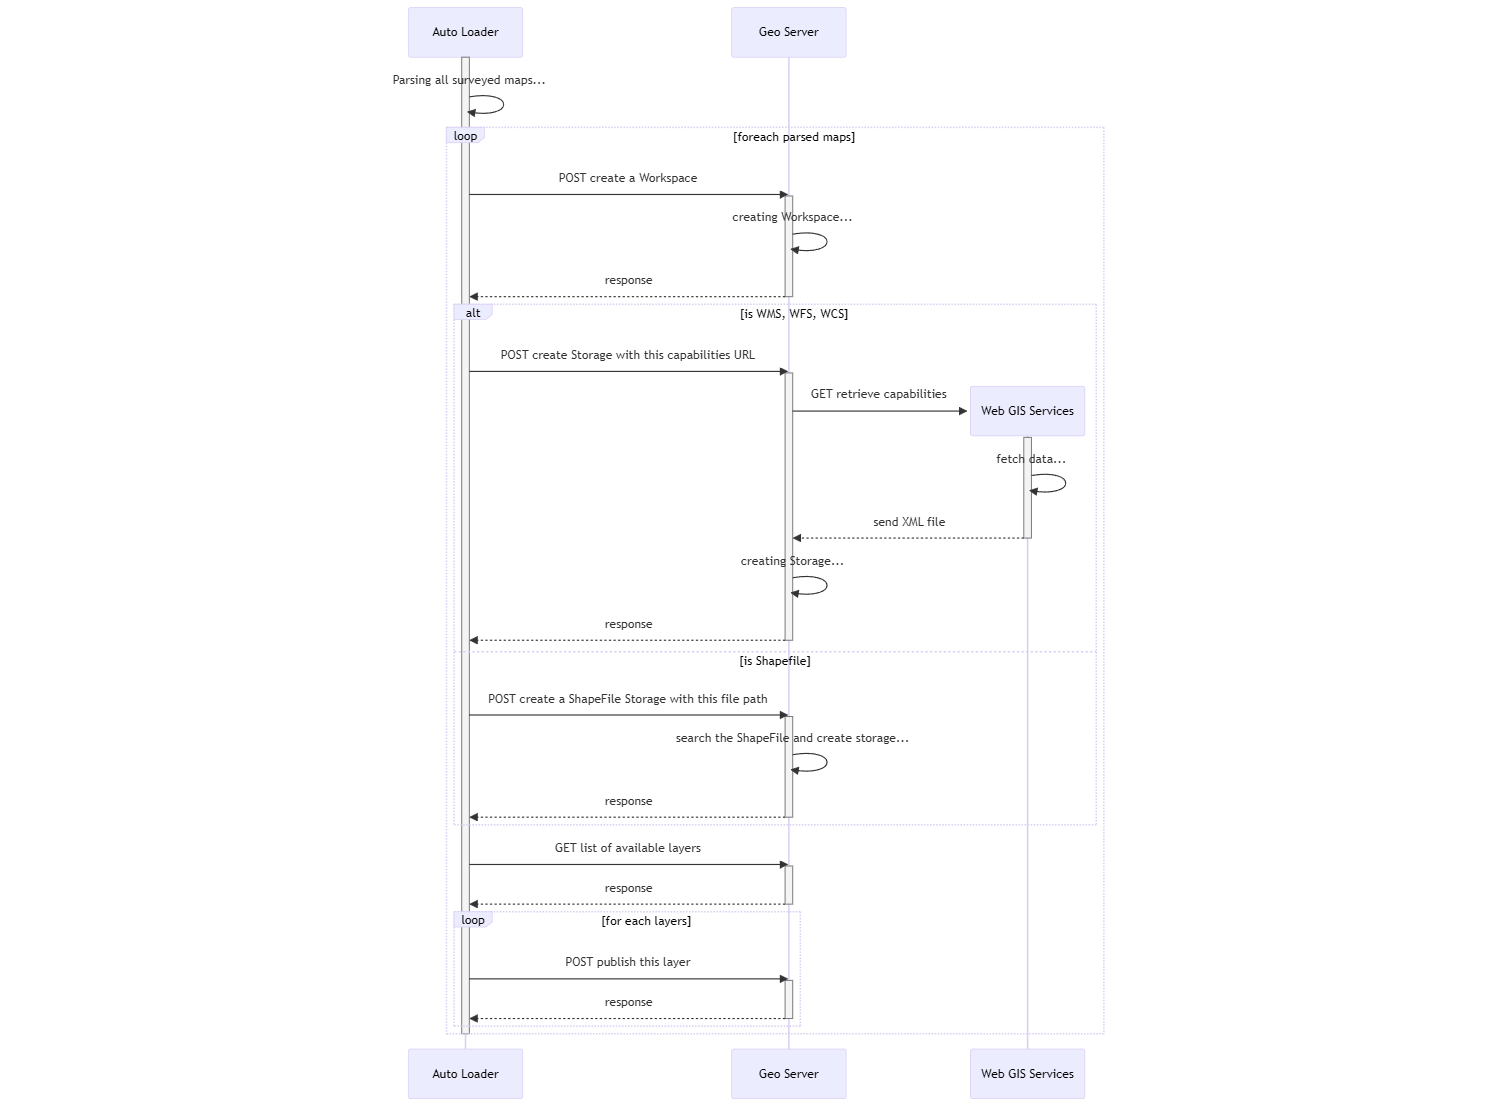
\includegraphics[width=2\textwidth]{Tesi/images/Capitolo6/BmsAutoloaderDiagramFix.png}}%      
      \caption{Ciclo di esecuzione del programma AutoLoader}
      \label{fig:BMSAutoloaderDiagram}      
\end{figure}
